

%% Normes de présentation visuelle 2018
%%
%% - grille de 8 unités de haut
%% - 1 mesure = 1/8 d'unité
%% - bande identitaire de 1 mesure placée au bas de la 7e unité
%% - logo haut de 4 mesures avec blancs de deux mesures en haut et
%%   en bas
%% - blanc équivalent à la largeur du blason à droite du logo
%% - bande or de la largeur du logo + blanc à droite
%%
%% Dimensions du logo UL
%%
%% hauteur: 128
%% largeur totale: 310
%% largeur blason: 100
%% valeur clé: (310 + 100)/128 = 3.2031125
%%
%% Dimensions de l'image
%%
%% hauteur: 55 mesures - 1pt (filet) = 54.9191919 mesures
%% largeur: 160mm
%% ratio largeur/hauteur: 160/77.23


\TPGrid{16}{64}
\textblockorigin{0mm}{0mm}
\setlength{\parindent}{0mm}
\setlength{\imageheight}{54.9191919\TPVertModule}
\setlength{\logoheight}{4\TPVertModule}
\setlength{\bandeorwidth}{3.203125\logoheight}
\setlength{\banderougewidth}{\paperwidth}
\addtolength{\banderougewidth}{-\bandeorwidth}
\setlength{\bandeorheight}{\TPVertModule}
\setlength{\banderougeheight}{\TPVertModule}
\setlength{\textwidth}{\paperwidth}
\addtolength{\textwidth}{-2\TPHorizModule}

\def\titlefmt{%
  \bfseries\fontsize{16}{16}\selectfont Big title}  
\def\subtitlefmt{%
  \mdseries\fontsize{11}{12}\selectfont Smaller subtitle
  \par}  
\def\authorfmt{%
  \bfseries\fontsize{12}{12}\selectfont {\scriptsize \mdseries Presented by \par} \\ 
  Student 1{\scriptsize \mdseries , \par}\\ 
  Student 2 {\scriptsize \mdseries et}\\
  Student 3\par}
\def\sigle{%
  \bfseries\fontsize{14}{14}\selectfont ABC-1234}   

%%%
%%% Page de titre
%%%

\begin{frame}[plain]
  %% bandeau identitaire
  \begin{textblock*}{\paperwidth}[0,1](0mm,56\TPVertModule)
    \textcolor{ulgray_red}{\rule{\banderougewidth}{\banderougeheight}}% % bande rouge
    \textcolor{ulgray_gold}{\rule{\bandeorwidth}{\bandeorheight}}           % bande or
  \end{textblock*}

  %% logo UL
  \begin{textblock*}{\bandeorwidth}(\banderougewidth,58\TPVertModule)
    
\includegraphics[height=\logoheight,keepaspectratio=true]{img/ul_logo_mono.png}
  \end{textblock*}

  %% image de fond
  \begin{textblock*}{\paperwidth}(0mm,0mm)
    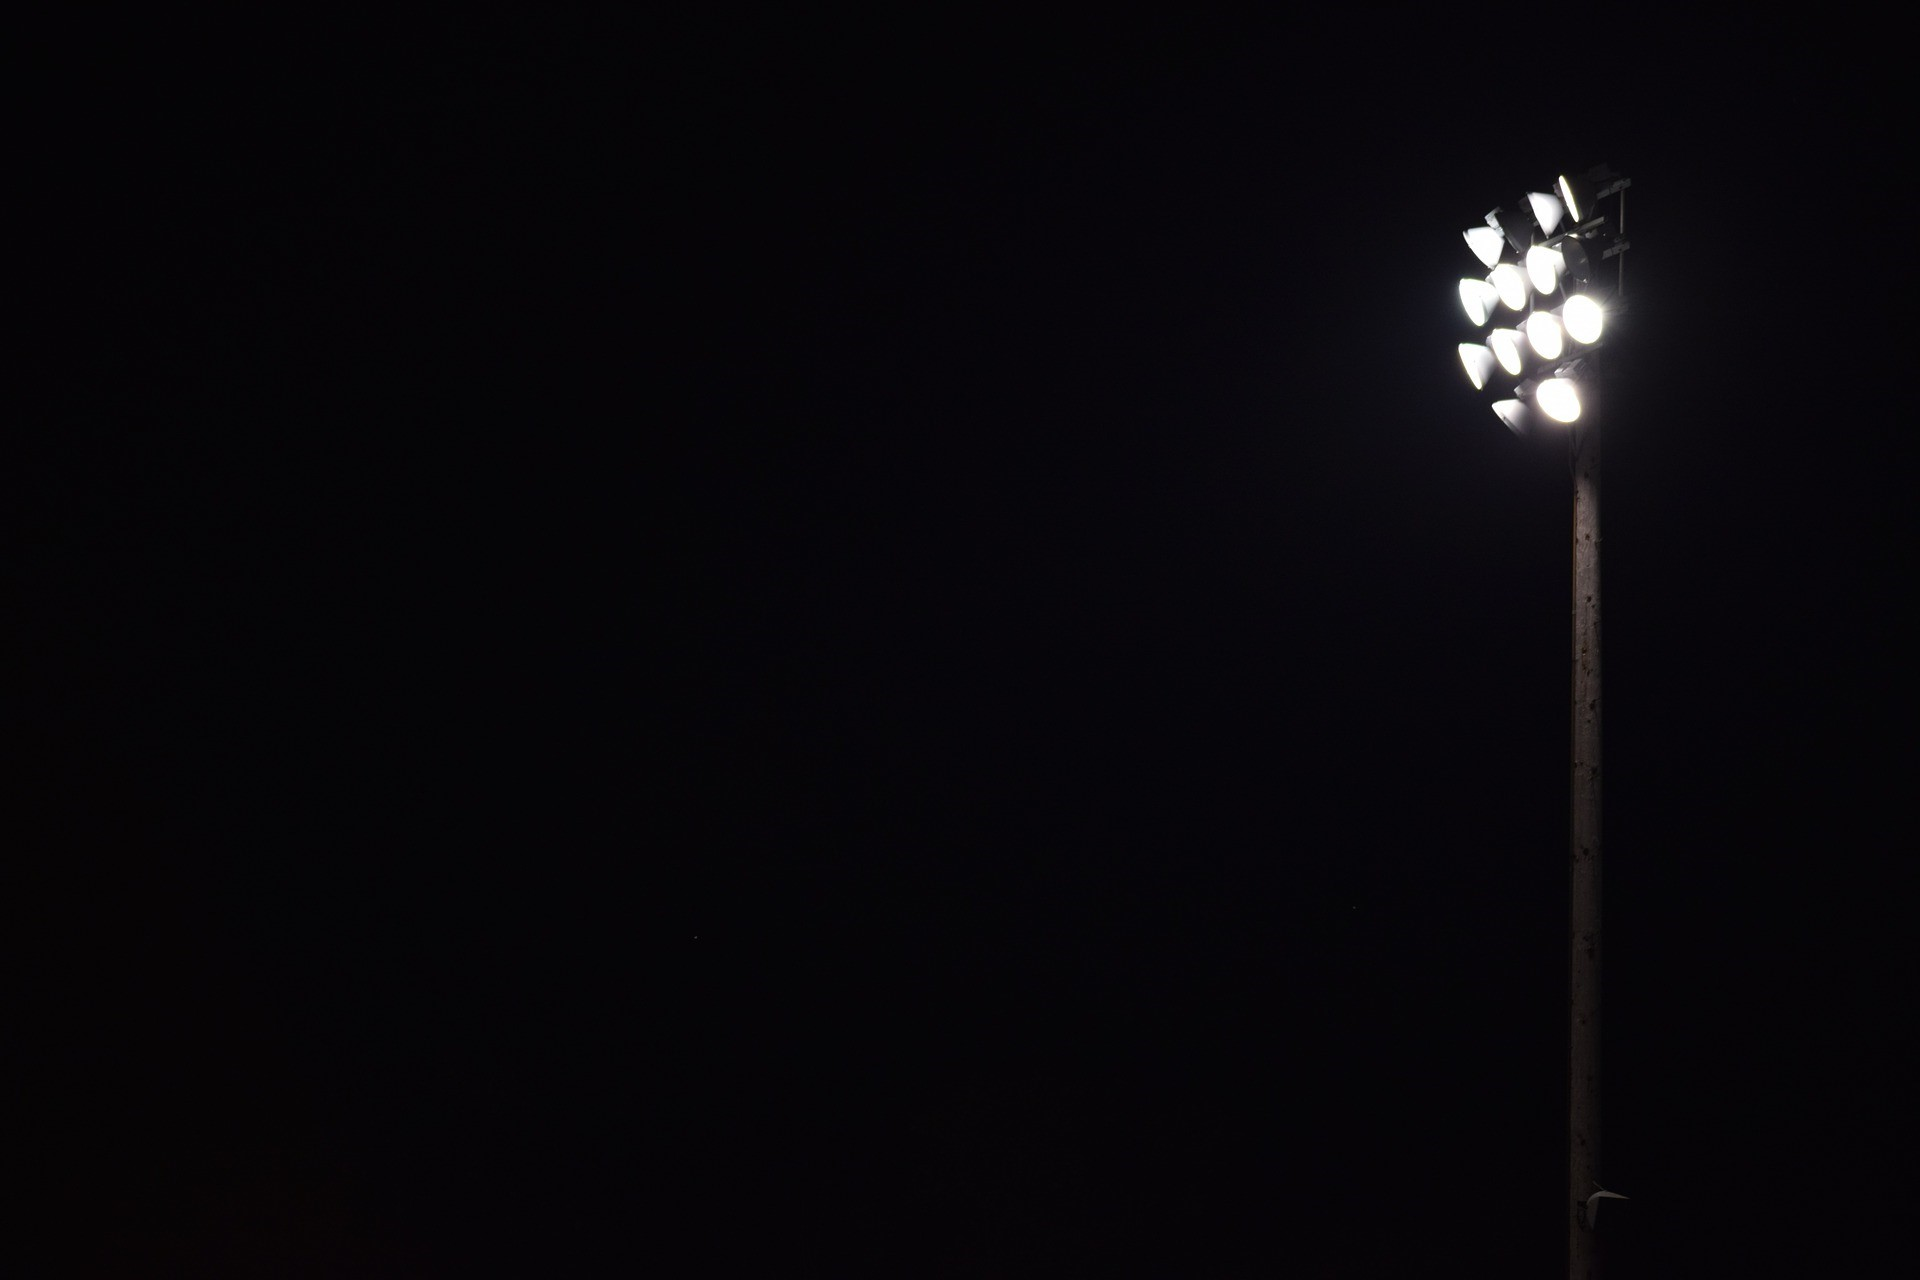
\includegraphics[height=\imageheight,width=\paperwidth]{img/fond_lumiere_stade.jpg}
  \end{textblock*}

  %% titre
  \begin{textblock*}{\banderougewidth}(0.8\TPHorizModule,4\TPVertModule)

    \textcolor{white}{\titlefmt}
  \end{textblock*}

  %% sous-titre (premiers pas)
  \begin{textblock*}{\banderougewidth}(0.8\TPHorizModule,9\TPVertModule)
    %\bidicontour{black}{\textcolor{white}{
    \textcolor{white}{\subtitlefmt}
    %}}
  \end{textblock*}
  
   %% auteurs
  \begin{textblock*}{\textwidth}(0.8\TPHorizModule,23\TPVertModule)
    \textcolor{white}{\authorfmt}
  \end{textblock*}

%  %% class
%   \begin{textblock*}{\textwidth}(0.8\TPHorizModule,44\TPVertModule)
%     \classfmt
%   \end{textblock*}
  
   %% sigle
  \begin{textblock*}{\textwidth}(0.8\TPHorizModule,46\TPVertModule)
    \textcolor{white}{\sigle}
  \end{textblock*}
  
  %% date
  \begin{textblock*}{\textwidth}(0.8\TPHorizModule,50\TPVertModule)
    \textcolor{white}{\today}
  \end{textblock*}
\end{frame}